% !TEX root = presentation.tex
	\begin{frame}
		\frametitle{Geometry}
		\todo[inline]{Bezier and Bernstein recap/why cubic?}

	\end{frame}

	\begin{frame}
		\frametitle{Geometry}
		\todo[inline]{How do you create the PN triangle geometrically}
	\end{frame}

	\begin{frame}
		\frametitle{Normals}
		\todo[inline]{How do you create the PN triangle normals}
	\end{frame}

	\begin{frame}
		\frametitle{Normals}
		\todo[inline]{Quadratic why no linear / cubic}
	\end{frame}

	\begin{frame}
		\frametitle{Level Of Detail}
		\todo[inline]{Barycentric coordinates recap}
	\end{frame}	

	\begin{frame}
		\frametitle{Level Of Detail}
		\todo[inline]{LOD verhaal}
		\begin{columns}
			\begin{column}{0.25\textwidth}
				\begin{center}
						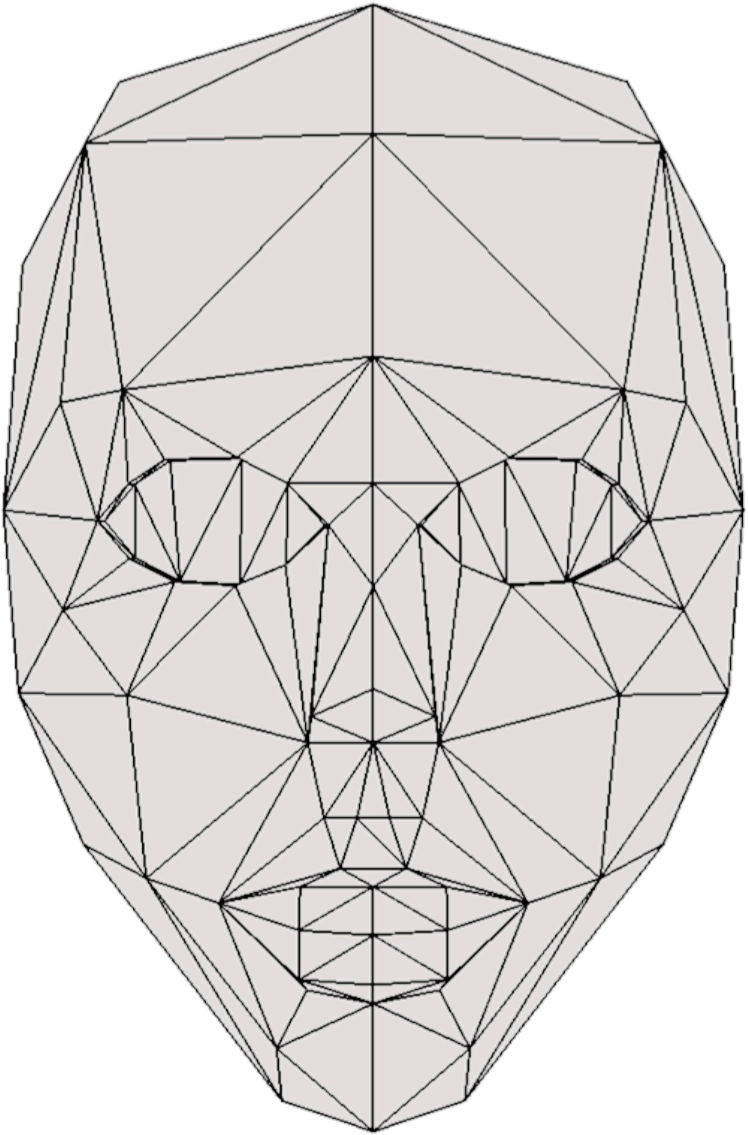
\includegraphics[width=\textwidth]{./img/0_intro/00_results_orange_1.png}	
				\end{center}	
			\end{column}
			\begin{column}{0.25\textwidth}
				\begin{center}
						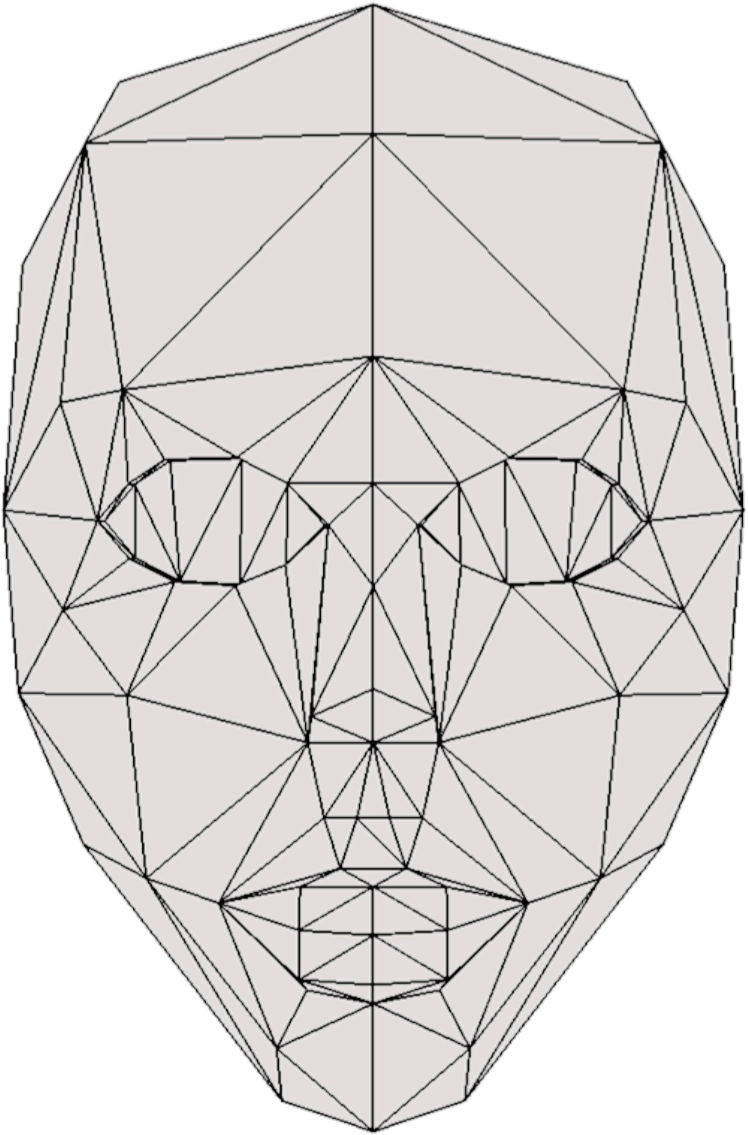
\includegraphics[width=\textwidth]{./img/0_intro/00_results_orange_1.png}	
				\end{center}	
			\end{column}
			\begin{column}{0.25\textwidth}
				\begin{center}
						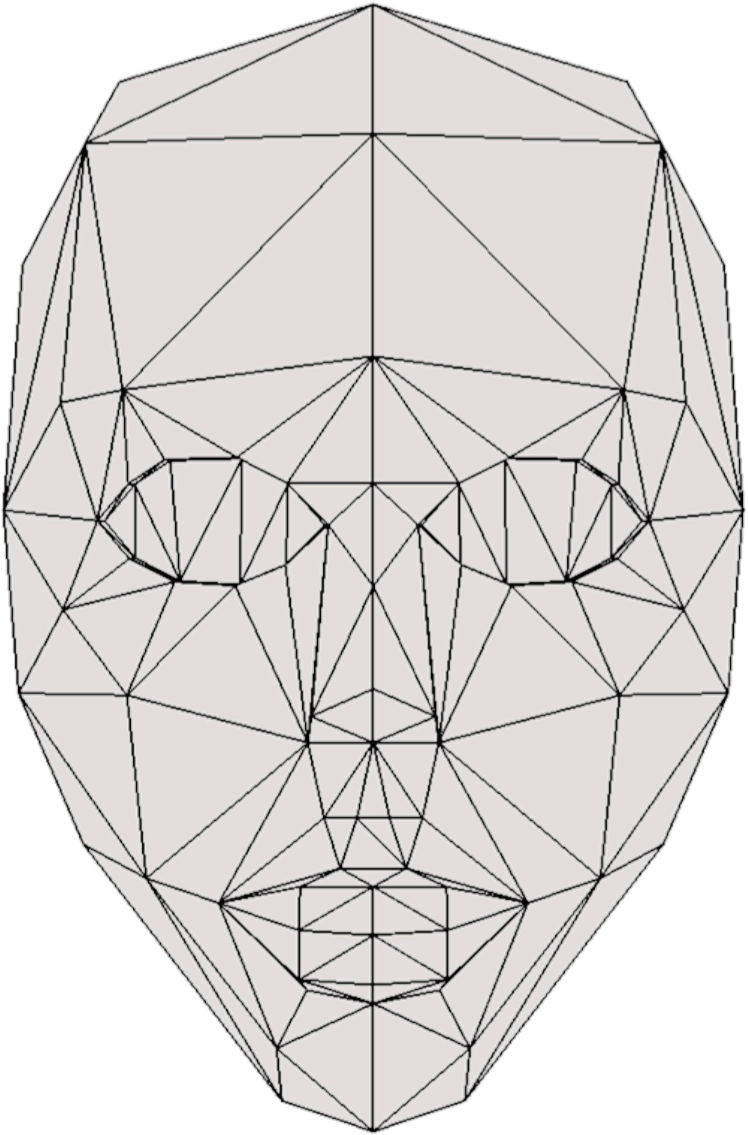
\includegraphics[width=\textwidth]{./img/0_intro/00_results_orange_1.png}	
				\end{center}	
			\end{column}
			\begin{column}{0.25\textwidth}
				\begin{center}
						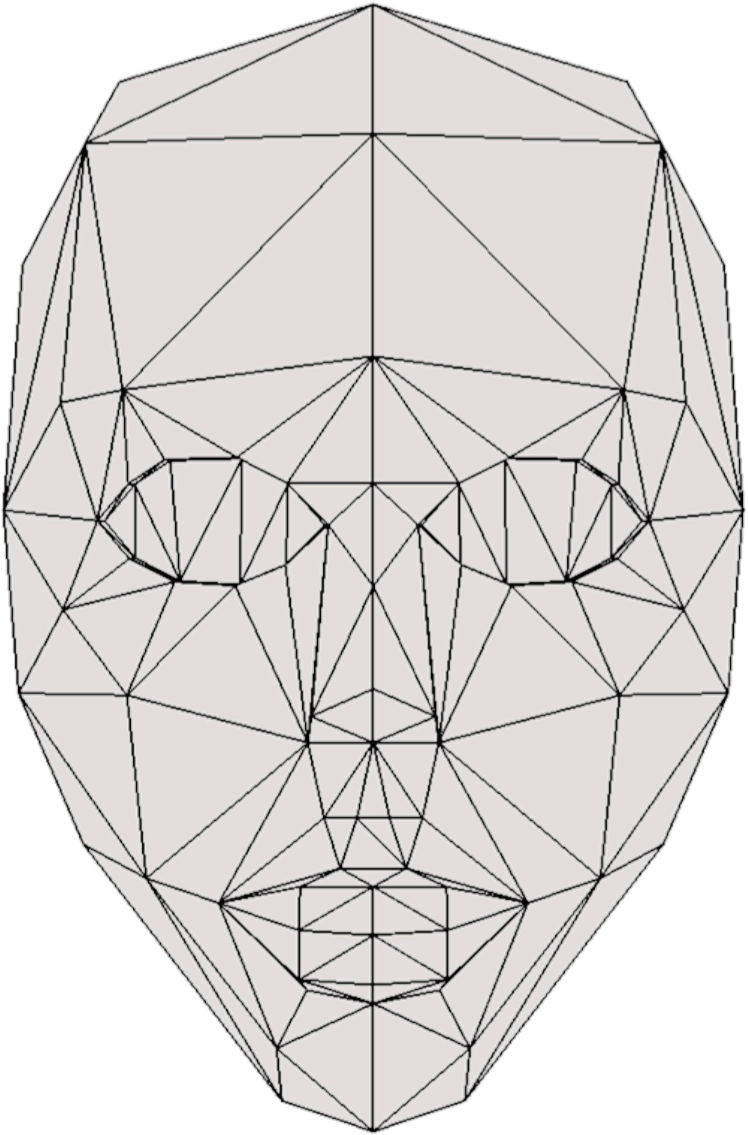
\includegraphics[width=\textwidth]{./img/0_intro/00_results_orange_1.png}	
				\end{center}	
			\end{column}
		\end{columns}
	\end{frame}	

	\begin{frame}
		\frametitle{Construction}
		\todo[inline]{The steps. Recap of everything construct geometry and normals and evaluate less (low lod) or more points (high lod)}
	\end{frame}	